\documentclass[letterpaper,twocolumn,10pt]{article}
\usepackage{usenix2019_v3}

\usepackage{url}
\usepackage{breakurl}
\def\UrlBreaks{\do\/\do-} %hack to force url breaks on "-" in references
% \usepackage[breaklinks, colorlinks]

% \usepackage[colorlinks,
	% linkcolor={[rgb]{0,0,0.4}},
	% urlcolor ={[rgb]{0,0,1}}, 
    % citecolor={[rgb]{0,0,0.4}}, 
    % ]{hyperref}

% \usepackage{hyperref}
% \renewcommand{\sectionautorefname}{\S}
% \renewcommand{\subsectionautorefname}{\S}
% \renewcommand{\subsubsectionautorefname}{\S}

\usepackage[ruled,vlined,linesnumbered]{algorithm2e}
\usepackage{comment}
\usepackage{soul, color}
\usepackage{graphicx}
\usepackage{caption}
\usepackage{subcaption}
\usepackage{threeparttable}
\usepackage{multirow}
\usepackage{booktabs}
\usepackage{verbatim}
\usepackage{epstopdf}
\usepackage{rotating}
\usepackage{listings}
\usepackage{listing}
\usepackage{paralist}
\usepackage{arydshln}
\let\labelindent\relax
\usepackage{enumitem,amssymb}
\usepackage{algpseudocode}% http://ctan.org/pkg/algorithmicx
\usepackage{balance}
\usepackage{endnotes}
\usepackage{xspace}
\usepackage{times}
\usepackage{amsfonts}
\usepackage{pifont}
\usepackage{wasysym}
\usepackage{tikz}
\usepackage{cite}

% to prevent "\pdfendlink ended up in different nesting level than \pdfstartlink" error.
\let\oldbibitem\bibitem
\def\bibitem{\vfill\oldbibitem}

\newcommand{\Tstrut}{\rule{0pt}{2.6ex}}         % = `top' strut
\newcommand{\Bstrut}{\rule[-0.9ex]{0pt}{0pt}}   % = `bottom' strut

\newcommand{\etc}{\textit{etc.}}
\newcommand{\ie}{\textit{i.e.}}
\newcommand{\tick}{\ding{51}}
\newcommand{\cross}{\ding{55}}

\graphicspath{{./figs/}}

%-------------------------------------------------------------------------------
\begin{document}
%-------------------------------------------------------------------------------

\date{}

\title{Title}
\author{}

\maketitle
\pagestyle{plain}

\begin{abstract}
	\begin{abstract}
abstract
\end{abstract}

\end{abstract}

\section{Introduction}
\label{s:intro}

\begin{figure}[h]
	\centering
	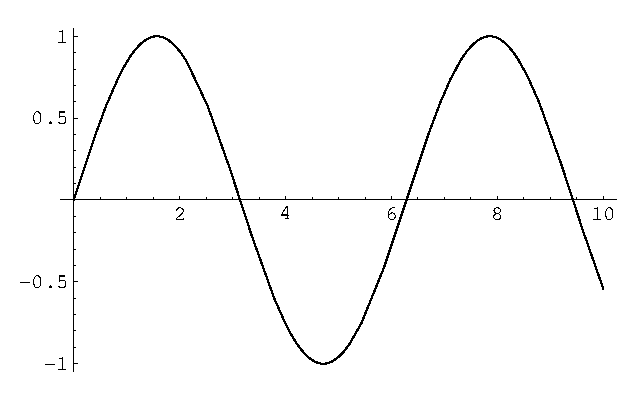
\includegraphics[width=0.8\linewidth]{sample}
	\caption{Sample}
	\label{f:sample}
\end{figure}

see this~\cite{latex}
\section{Background}
\label{s:backg}

\input{overview}
\section{Design}
\label{s:design}

\section{Evaluation}
\label{s:eval}

\input{discussion}
\section{Related work}
\label{s:relwk}
\section{Conclusion}
\label{s:conclusion}

% \section{Acknowledgment}
\label{s:ack}



% \bibliographystyle{abbrv}
\bibliographystyle{plain}
\bibliography{references}

% \appendix
% \section{Appendix}

This should be Appendix A!


\end{document}
